
% file that contains all the usepackages etc...
% ---------- Titelblad Masterproef Faculteit Wetenschappen -----------
% Dit document is opgesteld voor compilatie met pdflatex.  Indien je
% wilt compileren met latex naar dvi/ps, dien je de figuren naar
% (e)ps-formaat om te zetten.
%                           -- december 2012
% -------------------------------------------------------------------
\RequirePackage{fix-cm}
\documentclass[12pt,a4paper,oneside]{article}

% --------------------- In te laden pakketten -----------------------
% Deze kan je eventueel toevoegen aan de pakketten die je al inlaadt
% als je dit titelblad integreert met de rest van thesis.
% -------------------------------------------------------------------
\usepackage{graphicx,xcolor,textpos}
\usepackage{helvet}

% -------------------- Pagina-instellingen --------------------------
% Indien je deze wijzigt, zal het titelblad ook wijzigen.  Dit dien je
% dan manueel aan te passen.
% --------------------------------------------------------------------

\topmargin -10mm
\textwidth 160truemm
\textheight 240truemm
\oddsidemargin 0mm
\evensidemargin 0mm

% ------------------- textpos-instellingen ---------------------------
% Enkele andere instellingen voor het voorblad.
% --------------------------------------------------------------------

\definecolor{green}{RGB}{172,196,0}
\definecolor{bluetitle}{RGB}{29,141,176}
\definecolor{blueaff}{RGB}{0,0,128}
\definecolor{blueline}{RGB}{82,189,236}
\setlength{\TPHorizModule}{1mm}
\setlength{\TPVertModule}{1mm}



%----------------------- Custom stuff -------------------------------

\graphicspath{./}
\usepackage{makeidx}
\index{hoofd}
\makeindex
\usepackage{amsmath}
%\usepackage[dutch]{babel}
\usepackage[english]{babel}

\usepackage{hyperref}
\usepackage{graphicx}
\usepackage{caption}
\usepackage{subcaption}
\usepackage{amssymb}

\usepackage[toc,page]{appendix}



%------------------------ Plot packages ----------------------------
\usepackage{tikz}
\usepackage{pgfplots}

\usepackage{pgf}
\usepackage{units}
\usepackage{metalogo}



% -------------------Matlab code----------------------------------

\usepackage{listings}
\usepackage{color} %red, green, blue, yellow, cyan, magenta, black, white
\definecolor{mygreen}{RGB}{28,172,0} % color values Red, Green, Blue
\definecolor{mylilas}{RGB}{170,55,241}



% ------------------ Packages Matthias -----------------------

\usepackage{placeins}
\usepackage[normalem]{ulem}
\useunder{\uline}{\ul}{}
\usepackage{tabu}



\title{Genetic Algorithms and Evolutionary Computing \\ Project}
\author{ Jasper Hawinkel \& Matthias Baeten }
\date{ 11 january 2016}

% source code listing
\lstset{language=Matlab,%
    %basicstyle=\color{red},
    breaklines=true,%
    morekeywords={matlab2tikz},
    keywordstyle=\color{blue},%
    morekeywords=[2]{1}, keywordstyle=[2]{\color{black}},
    identifierstyle=\color{black},%
    stringstyle=\color{mylilas},
    commentstyle=\color{mygreen},%
    showstringspaces=false,%without this there will be a symbol in the places where there is a space
    numbers=left,%
    numberstyle={\tiny \color{black}},% size of the numbers
    numbersep=9pt, % this defines how far the numbers are from the text
    %emph=[1]{for,end,break},emphstyle=[1]\color{red}, %some words to emphasise
    %emph=[2]{word1,word2}, emphstyle=[2]{style},    
}


\begin{document}

	\maketitle
	\tableofcontents
	%\newpage
	

\section{Template TSP algorithm}

This section discusses the parameter tuning and experimentation with the provided Matlab template. The results gained with this algorithm are used in the following sections to compare them with the results from path representation.

\subsection{Parameter tuning}
 The template uses the adjecency representation with alternating edges crossover and inversion mutation. The parent selection mechanism is rank selection combined with elitism as survivor selection. Table \ref{table:question_2} shows the results of the performed parameter tuning on this algorithm. To produce these result the genetic algorithm was performed 10 times with each parameter setting on the \emph{rondrit067.tsp} file. The values shown in the last 2 columns (i.e. the best tour and the running time) are the averages of the results from those 10 runs. We started out with some standard parameters for the algorithm and then one by one tuned each parameter to find a good value. Then we combined the best results for each parameter. After some experimentation with this combination we settled on the parameters shown in the 3 to last row, with 20\% mutation chance, 50\% recombination and 10\% elitism.
 
\subsection{Results}
There are several interesting results that can be learned from table \ref{table:question_2}. Firstly, increasing the population only seams to have a minor impact on the execution time while there is significant benefit to the best tour found by the algorithm. For this particular problem, a population of 200-300 seems to be a reasonable trade-off between maximum fitness and execution time.

Secondly the chance of recombination seems to be a very important factor for the genetic algorithm, with a good choice of parameter resulting not only in better fitness evolution but also in reduced execution time compared to our initial value. The big reduction in execution time (almost 25\%) when going from 85\% recombination chance to 50\% indicates that a large part of the execution time is spent on recombination.

Thirdly, the parameters for mutation and elitism seem to have only a moderate impact on the performance of the genetic algorithm.

Lastly we tested the impact of loop detection on the genetic algorithm. This method removes loops of maximum 3 edges from all paths, increasing their fitness. From the results, it is clear that this method greatly improves maximum fitness with only a very small increase in execution time. The biggest downside to loop-detection is that this is a very problem specific method, limiting the range of problems the genetic algorithm can be applied to.

\begin{table}[!]
\centering
\begin{tabular}{ | l | l | l | l | l | l | l | l | }
\hline
{\ul \textbf{\#IND}} & {\ul \textbf{\#GEN}} & {\ul \textbf{PR. MUT}} & {\ul \textbf{PR. CROS}} & {\ul \textbf{ELITE}} & {\ul \textbf{LP DET}} & {\ul \textbf{DIST.}} & {\ul \textbf{TIME {[}sec{]}}} \\ \hline
	100 & 100 & 10\% & 85\% & 5\% & OFF & 14.21 & 10.91 \\ \hline
	150 & 100 & 10\% & 85\% & 5\% & OFF & 13.75 & 11.4 \\ \hline
	200 & 100 & 10\% & 85\% & 5\% & OFF & 13.23 & 12.65 \\ \hline
	300 & 100 & 10\%&  85\% & 5\% & OFF & 12.51 & 14.95 \\ \hline
	200 & 150 & 10\% & 85\% & 5\% & OFF & 12.25 & 20.03 \\ \hline
	200 & 200 & 10\% & 85\% & 5\% & OFF & 11.57 & 26.6 \\ \hline
	200 & 150 & 20\% & 85\% & 5\% & OFF & 12.33 & 21.95 \\ \hline
	200 & 150 & 30\% & 85\% & 5\% & OFF & 12.22 & 22.25 \\ \hline
	200 & 150 & 10\% & 80\% & 5\% & OFF & 11.63 & 18.64 \\ \hline
	200 & 150 & 10\% & 70\% & 5\% & OFF & 10.53 & 17.63 \\ \hline
	200 & 150 & 10\%& 60\% & 5\% & OFF & 9.49 & 17.39 \\ \hline
	200 & 150 & 10\% & 50\% & 5\% & OFF & 8.98 & 16.43 \\ \hline
	200 & 150 & 10\% & 85\% & 5\% & OFF & 9.1 & 17.46 \\ \hline
	200 & 150 & 10\% & 85\% & 10\% & OFF & 8.64 & 15.79 \\ \hline
	200 & 150 & 10\% & 85\% & 15\% & OFF & 8.85 & 16.04 \\ \hline
	200 & 200 & 20\% & 50\% & 5\% & OFF & 7.89 & 23.28 \\ \hline
	200 & 200 & 20\% & 50\% & 10\% & OFF & 7.38 & 21.56 \\ \hline
	200 & 150 & 20\% & 50\% & 10\% & OFF & 8.77 & 15.98 \\ \hline
	200 & 200 & 20\% & 50\% & 10\% & ON & 4.83 & 21.71 \\ \hline
	200 & 150 & 20\% & 50\% & 10\% & ON & 4.99 & 16.63 \\ \hline
\end{tabular}
\caption{Table with the results of some parameter tuning of the default genetic algorithm. The template TSP problem with $67$ cities is used. The second to last column contains the averages of the most optimal fitness values (minimal tour distance) found. The last column contains the averages of the computation time of a run. \#IND = \#INDIVIDUALS, \#GEN = \#GENERATIONS, PR. MUT = MUTATION PROBABILITY, PR. CROS = CROSSOVER PROBABILITY, LP DET = LOOP DETECTION, DIST = OPTIMAL DISTANCE. }
\label{table:question_2}
\end{table}

	

\section{Path Representation}

In this section an adjusted version of the existing genetic algorithm will be studied. The tours in the Traveling Salesman Problem will not be represented anymore by the adjacency representation. The path representation will be used instead. The $i$th element of the path representation denotes the $i$th city visited. This representation needs appropriate recombination and mutation operators. We chose to use the order crossover operator as recombination operator. For mutation we chose to use the inversion operator. 
\newline
\newline
The order crossover operator recombines the genes of two parents to produce two children. To produce the first offspring a randomly chosen segment of the first parent is copied into the offspring. Secondly information about the relative order of the second parent is used to make the representation of the first offspring complete. The second offspring is created in an analogous manner, with the parent roles reversed. The working process of the order crossover operator is shown below:

\begin{enumerate}
  \item Choose two crossover points at random, and copy the segment between them from the first parent into the first offspring.
  \item Starting from the second crossover point in the second parent, and copy the remaining unused numbers into the first offspring in the order that they appear in the second parent.
  \item Create the second offspring in an analogous manner, with the parent roles reversed.
\end{enumerate}

The used mutation operator is the inversion mutation operator. This operator works by randomly selecting two positions in the chromosome and reversing the order in which the values appear between those positions. For more information about these operators we refer to \cite{handboek}. The implementation of the order crossover operator is shown in the appendices. The code for evaluating the fitness of candidate solutions in path representation is also shown in the appendices. The path representation and the inversion mutation operator were already implemented in the template Matlab program for the TSP.
\newline
\newline
Now we will perform some parameter tuning to identify proper combinations of the parameters. Remark that genetic algorithms are stochastic. That is why we can not draw any conclusions about the quality of the genetic algorithm from a single run. Therefore multiple runs will be used to estimate the quality of the genetic algorithm for a certain set of algorithm parameters. For every run the computation time and the best candidate solution found are stored. The computations times and the fitness values of the most optimal solutions found are then averaged over the amount of runs. The results of the parameter tuning process are shown in table \ref{table:question_3}.
\newline
\newline
We started the parameter tuning process by using the default parameters used in the template program. These default parameters are shown in the second row of table \ref{table:question_3}. Next we studied every parameter separately by only adjusting the value of one parameters and using the default values for the other parameters. In that way we can find the optimal value for each parameter separately. At the end we then combine the optimal parameter values and hopefully this will give us the optimal set of parameters. As we already expected, increasing the population size and the number of generations improves the results. The disadvantage is that the computation time (and probably the amount of memory needed) increases also. It is clear that here some sort of trade-off has to be made between solution quality and CPU time (and memory needed). The optimal value for the probability of mutation seems to lie around $8\%$ and the optimal value for the probability of recombination seems to lie around $80\%$. The optimal proportion of elite seems to lie around $15\%$. As we expected the results with loop detection are much better than without. With loop detection no significantly more CPU time is needed than without. So if loop detection is implemented, you should always use it.
\newline
\newline
In the four last columns of table \ref{table:question_3} the optimal values for the mutation and crossover probability and elite proportion are used. The combined optimal values indeed result in very good results. It seems like it is more optimal to take the number of individuals equal to the number of generators instead of only half. Increasing the number of individuals does not double the amount of computation time in contrast to the number of generations. 


% TO MAKE THIS TABLE EASY: SEE GOOGLE: LATEX CREATE TABLES ONLINE !!!!!!!!!
% Please add the following required packages to your document preamble:
% \usepackage[normalem]{ulem}
% \useunder{\uline}{\ul}{}
\begin{table}[!]
\centering
\begin{tabular}{|c|c|c|c|c|c|c|c|}
\hline
{\ul \textbf{\#IND}} & {\ul \textbf{\#GEN}} & {\ul \textbf{PR. MUT}} & {\ul \textbf{PR. CROS}} & {\ul \textbf{ELITE}} & {\ul \textbf{LP DET}} & {\ul \textbf{DIST.}} & {\ul \textbf{TIME {[}sec{]}}} \\ \hline
\textbf{50}          & \textbf{100}         & \textbf{5 \%}          & \textbf{95 \%}          & \textbf{5 \%}        & \textbf{OFF}          & \textbf{10.99}       & \textbf{10.80}                 \\ \hline
\textbf{100}         & df                   & df                     & df                      & df                   & df                    & \textbf{9.962}        & \textbf{12.56}                \\ \hline
\textbf{200}         & df                   & df                     & df                      & df                   & df                    & \textbf{9.425}        & \textbf{15.09}                \\ \hline
\textbf{500}         & df                   & df                     & df                      & df                   & df                    & \textbf{8.926}        & \textbf{25.18}                \\ \hline
df                   & \textbf{200}         & df                     & df                      & df                   & df                    & \textbf{8.919}        & \textbf{21.83}                \\ \hline
df                   & \textbf{500}         & df                     & df                      & df                   & df                    & \textbf{6.721}        & \textbf{52.53}                \\ \hline
df                   & df                   & \textbf{0 \%}          & df                      & df                   & df                    & \textbf{10.95}       & \textbf{10.75}                \\ \hline
df                   & df                   & \textbf{8 \%}          & df                      & df                   & df                    & \textbf{10.76}       & \textbf{10.76}                \\ \hline
df                   & df                   & \textbf{15 \%}         & df                      & df                   & df                    & \textbf{11.21}       & \textbf{11.08}                \\ \hline
df                   & df                   & df                     & \textbf{70 \%}          & df                   & df                    & \textbf{10.66}       & \textbf{9.499}                 \\ \hline
df                   & df                   & df                     & \textbf{80 \%}          & df                   & df                    & \textbf{10.54}       & \textbf{10.41}                \\ \hline
df                   & df                   & df                     & \textbf{90 \%}          & df                   & df                    & \textbf{10.70}       & \textbf{10.74}                \\ \hline
df                   & df                   & df                     & \textbf{100 \%}         & df                   & df                    & \textbf{10.86}       & \textbf{10.82}                \\ \hline
df                   & df                   & df                     & df                      & \textbf{0 \%}        & df                    & \textbf{15.61}       & \textbf{11.01}                \\ \hline
df                   & df                   & df                     & df                      & \textbf{10 \%}       & df                    & \textbf{10.17}       & \textbf{9.855}                 \\ \hline
df                   & df                   & df                     & df                      & \textbf{15 \%}       & df                    & \textbf{9.954}        & \textbf{9.787}                 \\ \hline
df                   & df                   & df                     & df                      & \textbf{20 \%}       & df                    & \textbf{10.14}       & \textbf{9.520}                 \\ \hline
df                   & df                   & df                     & df                      & \textbf{25 \%}       & df                    & \textbf{10.38}       & \textbf{9.661}                 \\ \hline
df                   & df                   & df                     & df                      & df                   & \textbf{ON}           & \textbf{7.020}        & \textbf{10.48}                \\ \hline
\textbf{100}         & \textbf{200}         & \textbf{8 \%}          & \textbf{80 \%}          & \textbf{15 \%}       & \textbf{OFF}          & \textbf{7.143}        & \textbf{22.82}                \\ \hline
\textbf{200}         & \textbf{200}         & \textbf{8 \%}          & \textbf{80 \%}          & \textbf{15 \%}       & \textbf{OFF}          & \textbf{6.394}        & \textbf{28.01}                \\ \hline
\textbf{100}         & \textbf{200}         & \textbf{8 \%}          & \textbf{80 \%}          & \textbf{15 \%}       & \textbf{ON}           & \textbf{5.357}        & \textbf{23.09}                \\ \hline
\textbf{200}         & \textbf{200}         & \textbf{8 \%}          & \textbf{80 \%}          & \textbf{15 \%}       & \textbf{ON}           & \textbf{4.932}        & \textbf{28.62}                \\ \hline
\end{tabular}
\caption{Table with the results of some parameter tuning of the genetic algorithm. A path representation is used with order crossover and inversion mutation. For every set of parameters 10 runs are calculated. The template TSP problem with $67$ cities is used. The second last column contains the averages of the most optimal fitness values (minimal tour distance) found. The last column contains the averages of the computation time of a run. \texttt{df} stands for 'default value'. In the boxes with a \texttt{df} statement the default value from the first row is used. \#IND = \#INDIVIDUALS, \#GEN = \#GENERATIONS, PR. MUT = MUTATION PROBABILITY, PR. CROS = CROSSOVER PROBABILITY, LP DET = LOOP DETECTION, DIST = OPTIMAL DISTANCE. }
\label{table:question_3}
\end{table}

\FloatBarrier
	

\section{Benchmark Problems}

In this section we will test the performance of our designed algorithm (path representation) using some larger benchmark problems. Again we tested the parameter values in table \ref{table:question_3}. And we came to the conclusion that the optimal parameter values found in table \ref{table:question_3} are also the optimal parameter values for larger benchmark problems. We executed the tests on the benchmark problem containing 380 cities (\texttt{bcl380.tsp}). It is certainly not that logical that the parameter values that are optimal for small size problems are also the optimal values for larger size problems. Now that we have found the optimal parameter settings for our genetic algorithm, we can use the algorithm to solve some large benchmark problems.
In figure \ref{fig:belgium_tour_4} you can see the results for the Belgium tour benchmark problem. It seems that the GA found the optimal solution very quickly. 
\newline
\newline
We also did a performance comparison of the original GA (adjacency representation) with the new designed GA (path representation). For both algorithms their optimal set of parameter values are used. In figure \ref{fig:adj_vraag4_off_gen} and \ref{fig:path_vraag4_off_gen} the results are shown with loop detection switched off. We see that the new designed GA finds a shorter optimal tour than the original GA. The disadvantage of the new designed GA is that it takes more computation time than the original GA. In figure \ref{fig:adj_vraag4_on_gen} and \ref{fig:path_vraag4_on_gen} the same experiment is done with loop detection switched on. Now both methods obtain approximately the same tour quality but the new designed GA takes again more CPU time. Notice that with the original GA in figure \ref{fig:adj_vraag4_on_gen} the fitness values are decreasing very fast at the beginning and after that they decrease rather slow.If we compare this behavior with the new GA in figure \ref{fig:adj_vraag4_on_gen} we see that with the new GA the fitness value decrease more gradually over the generation process. 
\newline
\newline
It seems that with loop detection switched on, the original GA and the new GA obtain the same tour quality, but the new GA needs more computation time . Without loop detection the new GA gives better results, but it takes more CPU time. Remark that with the original GA that the fitness value of the worst solution in the population set is always far away from the fitness values of the best and average solution. With the new designed GA these three values lie much closer together.

%\begin{figure}[!ht]
%  \centering
%    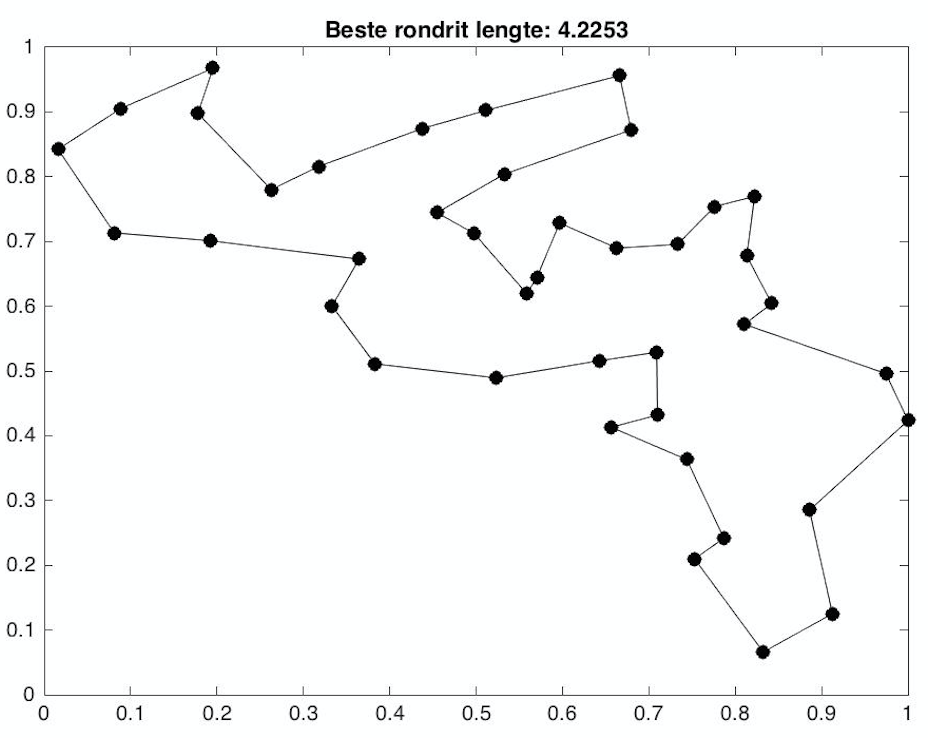
\includegraphics[width=0.5\textwidth]{../figures/figures_question_4/belgium_tour_path}
%      \caption{ There are }
%      \label{fig:belgium_path_4}
%\end{figure}

\begin{figure}[!]
\centering
\begin{subfigure}{.5\textwidth}
  \centering
  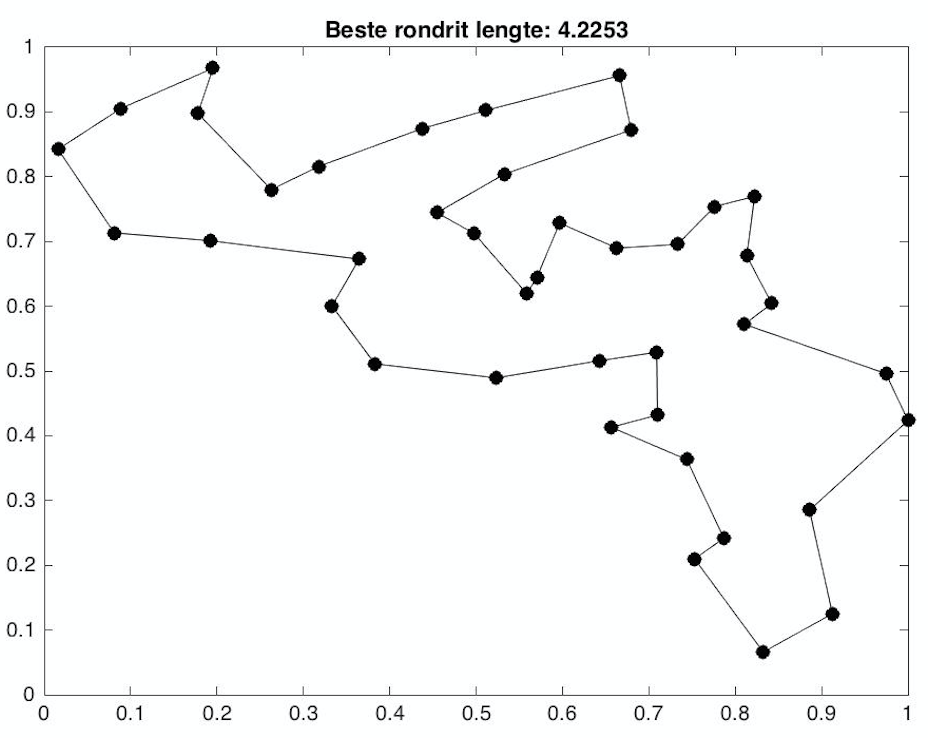
\includegraphics[width=.88\linewidth]{../figures/figures_question_4/belgium_tour_path}
  \caption{The most optimal tour found for the TSP problem. The distance of the tour is $4.2253$.\\ \ \\}
  \label{fig:belgium_tour_4_path}
\end{subfigure}%
\begin{subfigure}{.5\textwidth}
  \centering
  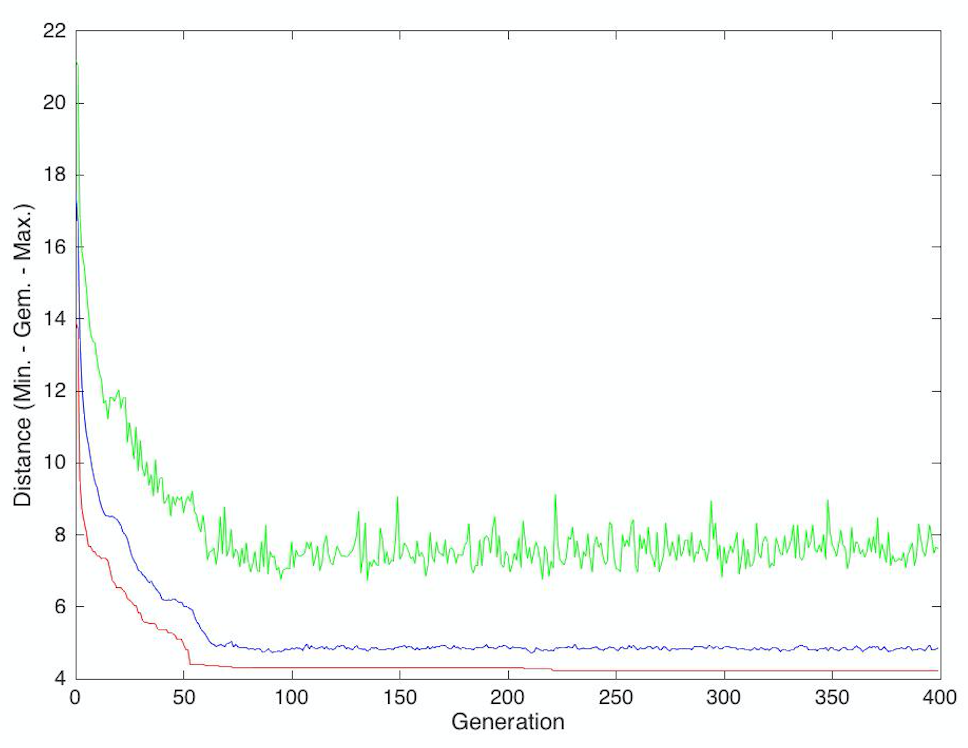
\includegraphics[width=.9\linewidth]{../figures/figures_question_4/belgium_tour_gen}
  \caption{The fitness values (tour distances) for the best(red), average(blue) and worst(green) candidate solution in every generation. \\}
  \label{fig:belgium_tour_4_gen}
\end{subfigure}
\caption{The benchmark TSP problem \texttt{belgiumtour.tsp} with 41 cities is solved here with path representation, order crossover and inversion mutation. The settings of the GA were \#IND = 400, \#GEN = 400, PR. MUT = $8\%$, PR. CROS = $80\%$, , ELITE = $15\%$, LP DET = ON.}
\label{fig:belgium_tour_4}
\end{figure}


\begin{figure}[!]
  \centering
    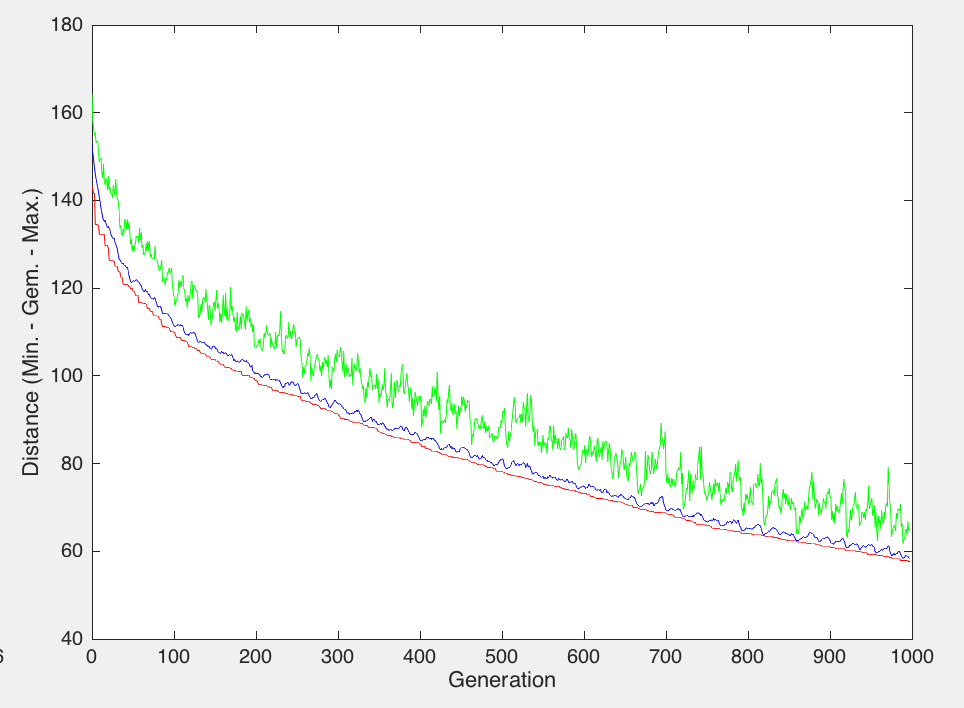
\includegraphics[width=0.6\textwidth]{../figures/figures_question_4/adj_vraag4_off_gen}
      \caption{The benchmark TSP problem \texttt{belgiumtour.tsp} with 380 cities is solved here with \textbf{adjacency representation (original GA)}. The optimal candidate solution is far away from the best solution. \textbf{The optimal tour distance found is $\mathbf{57.14}$ and the computation time needed was around 209 seconds}. \textbf{The optimal settings of the original GA were used}, namely PR. MUT = $10\%$, PR. CROS = $50\%$ , ELITE = $10\%$. 200 individuals and 1000 generations are used and \textbf{loop detection is switched off}. The fitness values (tour distances) for the best(red), average(blue) and worst(green) candidate solution in every generation.}
      \label{fig:adj_vraag4_off_gen}
\end{figure}

\begin{figure}[!]
  \centering
    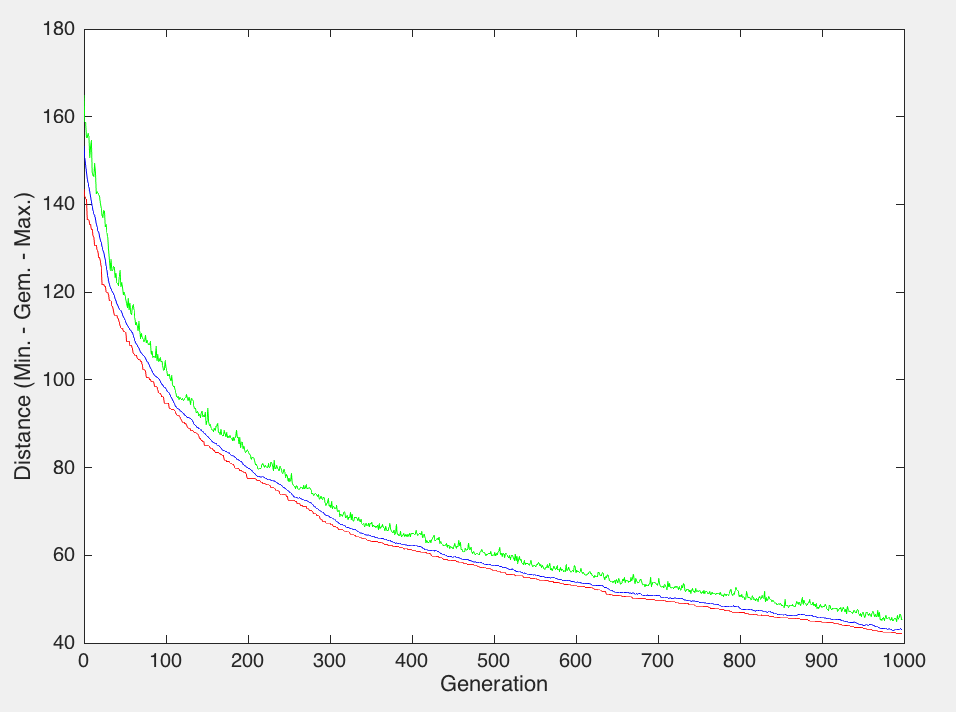
\includegraphics[width=0.6\textwidth]{../figures/figures_question_4/path_vraag4_off_gen}
      \caption{The benchmark TSP problem \texttt{belgiumtour.tsp} with 380 cities is solved here with \textbf{path representation (new designed GA)}. The optimal candidate solution is far away from the best solution. \textbf{The optimal tour distance found is $\mathbf{42.1}$ and the computation time needed was around 357 seconds}. \textbf{The optimal settings of the new designed GA were used}, namely PR. MUT = $8\%$, PR. CROS = $80\%$ , ELITE = $15\%$. 200 individuals and 1000 generations are used and \textbf{loop detection is switched off}. The fitness values (tour distances) for the best(red), average(blue) and worst(green) candidate solution in every generation.}
      \label{fig:path_vraag4_off_gen}
\end{figure}

\begin{figure}[!]
  \centering
    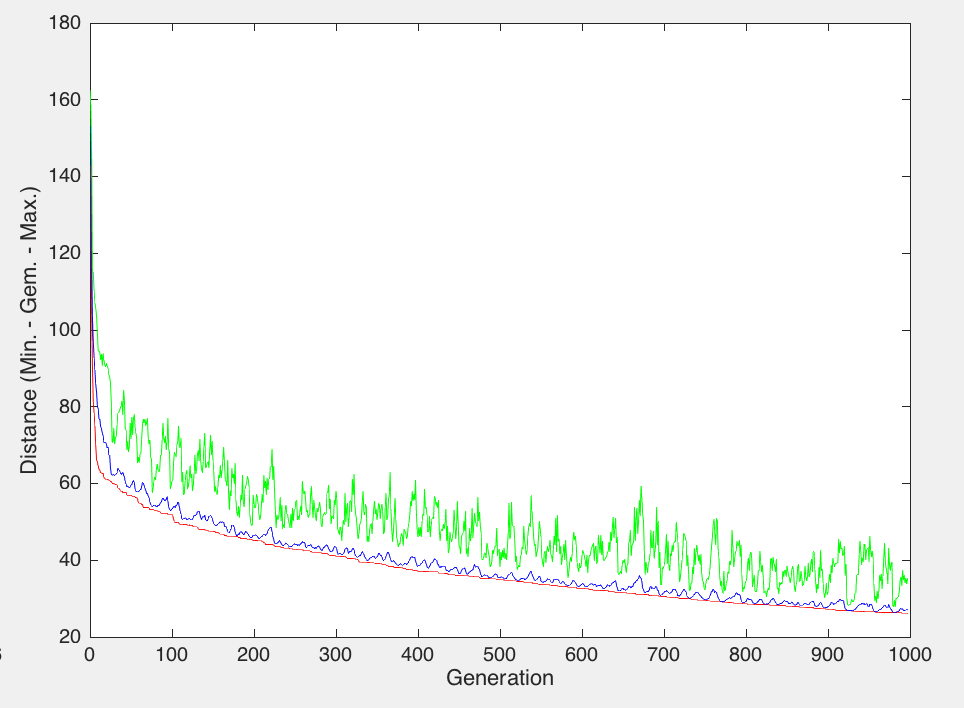
\includegraphics[width=0.6\textwidth]{../figures/figures_question_4/adj_vraag4_on_gen}
      \caption{The benchmark TSP problem \texttt{belgiumtour.tsp} with 380 cities is solved here with \textbf{adjacency representation (original GA)}. The optimal candidate solution is far away from the best solution. \textbf{The optimal tour distance found is $\mathbf{26.2}$ and the computation time needed was around 226 seconds}. \textbf{The optimal settings of the original GA were used}, namely PR. MUT = $10\%$, PR. CROS = $50\%$ , ELITE = $10\%$. 200 individuals and 1000 generations are used and \textbf{loop detection is switched on}. The fitness values (tour distances) for the best(red), average(blue) and worst(green) candidate solution in every generation.}
      \label{fig:adj_vraag4_on_gen}
\end{figure}

\begin{figure}[!]
  \centering
    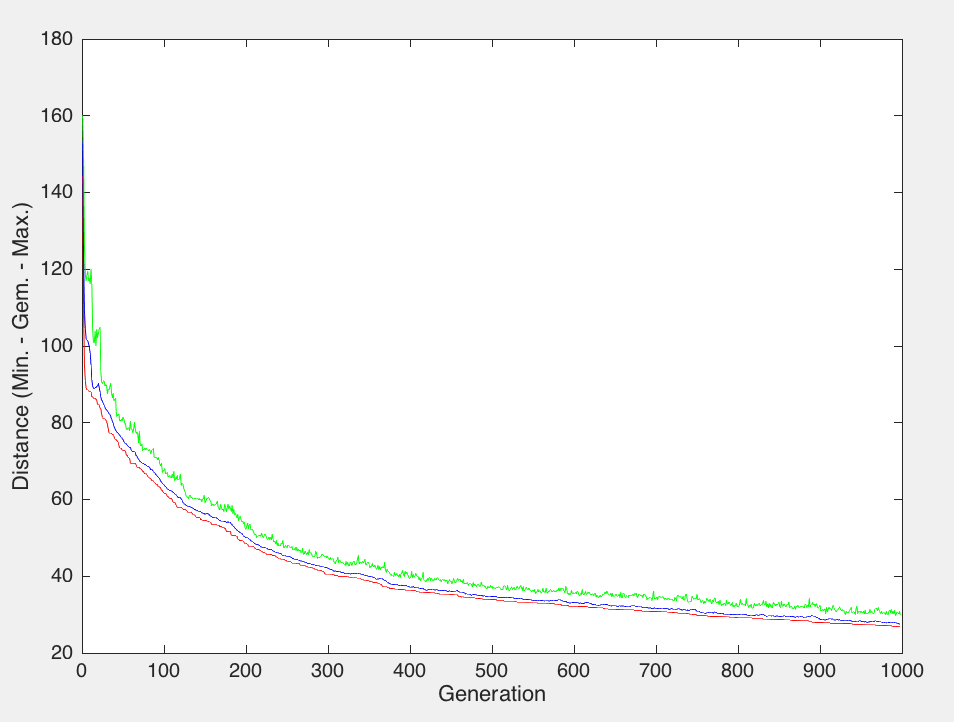
\includegraphics[width=0.6\textwidth]{../figures/figures_question_4/path_vraag4_on_gen}
      \caption{The benchmark TSP problem \texttt{belgiumtour.tsp} with 380 cities is solved here with \textbf{path representation (new designed GA)}. The optimal candidate solution is far away from the best solution. \textbf{The optimal tour distance found is $\mathbf{26.8}$ and the computation time needed was around 387 seconds}. \textbf{The optimal settings of the new designed GA were used}, namely PR. MUT = $8\%$, PR. CROS = $80\%$ , ELITE = $15\%$. 200 individuals and 1000 generations are used and \textbf{loop detection is switched on}. The fitness values (tour distances) for the best(red), average(blue) and worst(green) candidate solution in every generation.}
      \label{fig:path_vraag4_on_gen}
\end{figure}














%\begin{figure}[!]
%  \centering
%    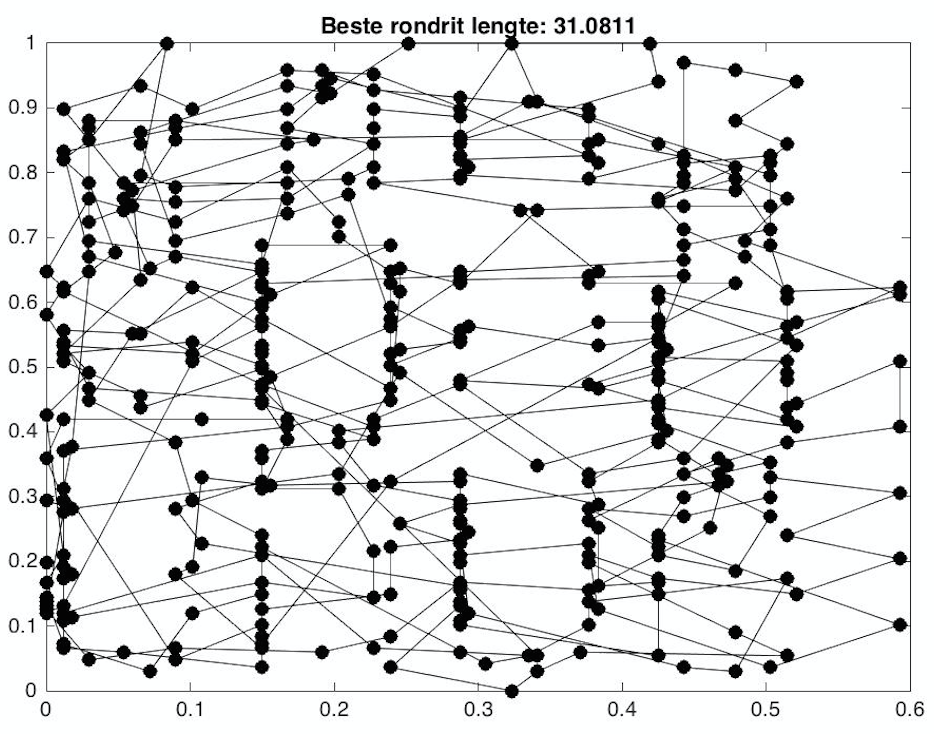
\includegraphics[width=0.7\textwidth]{../figures/figures_question_4/cities380_4_path}
%      \caption{The benchmark TSP problem \texttt{belgiumtour.tsp} with 380 cities is solved here with path representation, order crossover and inversion mutation. The optimal candidate solution is far away from the best solution. The settings of the GA were \#IND = 500, \#GEN = 500, PR. MUT = $8\%$, PR. CROS = $80\%$ , ELITE = $15\%$, LP DET = ON. The CPU time needed was 440 seconds.}
%      \label{fig:cities380_4_path}
%\end{figure}
%
%\begin{figure}[!]
%  \centering
%    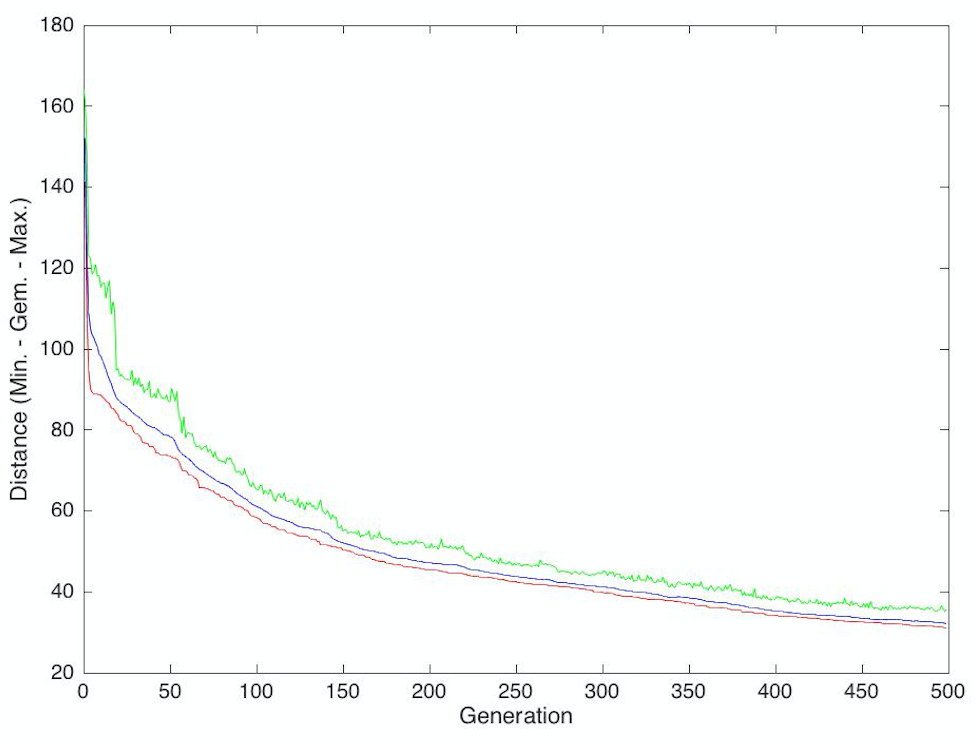
\includegraphics[width=0.7\textwidth]{../figures/figures_question_4/cities380_4_gen}
%      \caption{The fitness values (tour distances) for the best(red), average(blue) and worst(green) candidate solution in every generation. This figure corresponds to the problem solved in figure \ref{fig:cities380_4_path}}
%      \label{fig:cities380_4_gen}
%\end{figure}
%
%\begin{figure}[!]
%  \centering
%    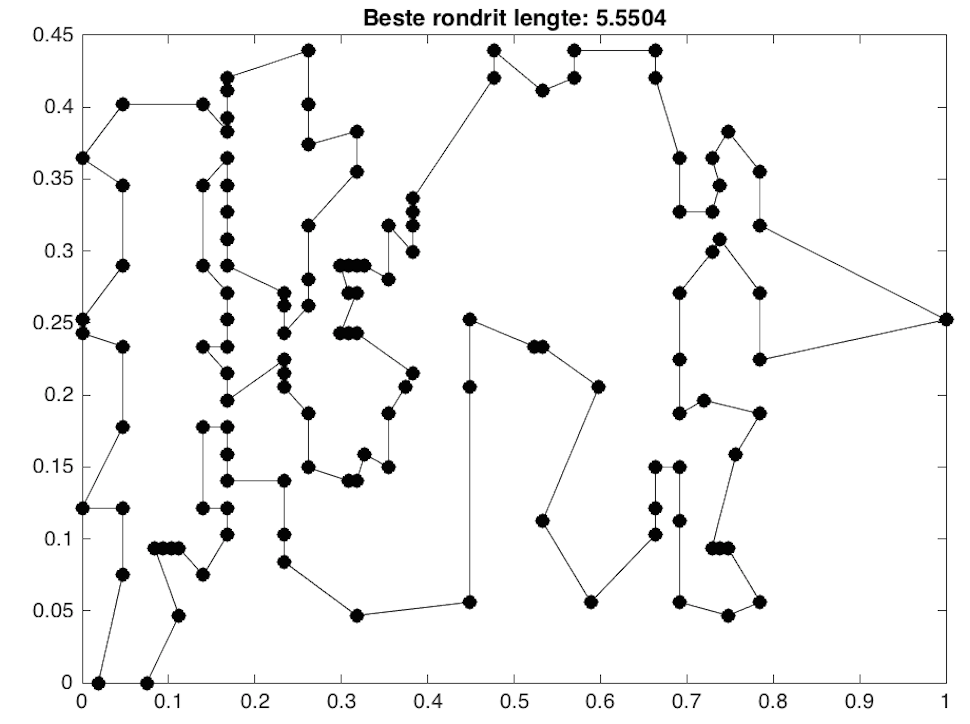
\includegraphics[width=0.7\textwidth]{../figures/figures_question_4/benchmark_131_path}
%      \caption{The benchmark TSP problem \texttt{xqf131.tsp} with 131 cities is solved here with path representation, order crossover and inversion mutation. The optimal candidate solution is very good. The settings of the GA were \#IND = 1000, \#GEN = 1000, PR. MUT = $8\%$, PR. CROS = $80\%$ , ELITE = $15\%$, LP DET = ON. The CPU time needed was 584 seconds.}
%      \label{fig:benchmark_131_path}
%\end{figure}
%
%\begin{figure}[!]
%  \centering
%    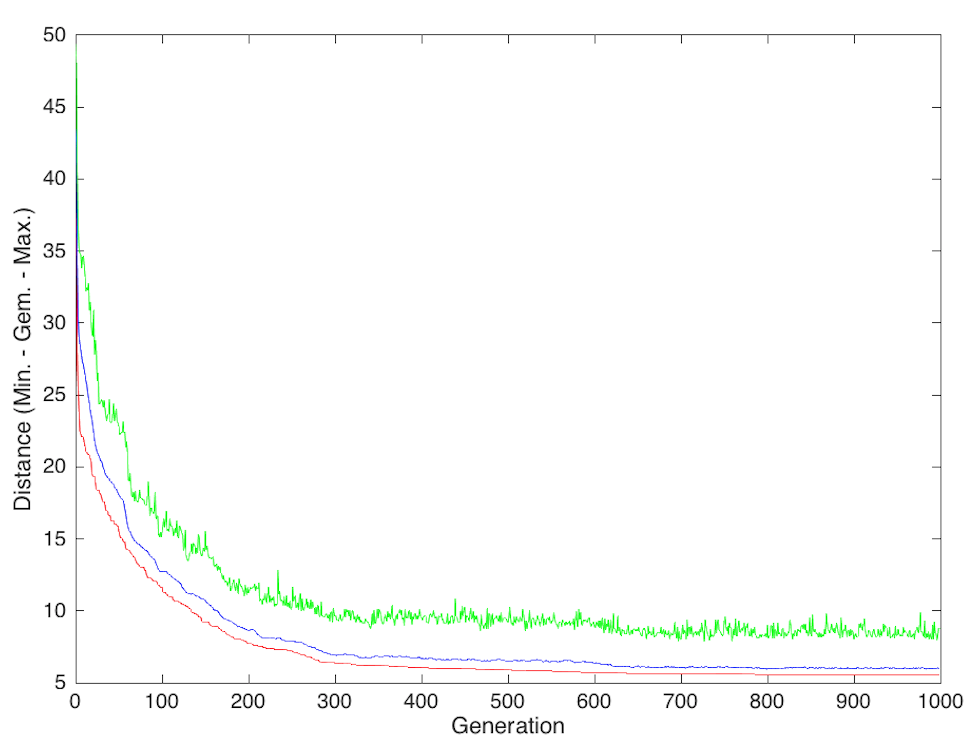
\includegraphics[width=0.7\textwidth]{../figures/figures_question_4/benchmark_131_gen}
%      \caption{The fitness values (tour distances) for the best(red), average(blue) and worst(green) candidate solution in every generation. This figure corresponds to the problem solved in figure \ref{fig:benchmark_131_path}}
%      \label{fig:benchmark_131_gen}
%\end{figure}



\FloatBarrier
	

\section{Alternative parent selection}
 This section will discuss two alternative forms of parent selection: tournament selection and fitness proportionate selection. 
 
 \subsection{Fitness proportionate selection}
 The fitness proportionate selection method assigns to each individual a probability of selection that is directly proportional to its fitness value. This is summed up in formula \ref{eq:fitness_prop}. Because the fitness function is to be minimised, the fitness values are inverted prior to calculating the probabilities. 
 \begin{equation} \label{eq:fitness_prop}
 P(i) = \dfrac{\dfrac{1}{f_i}}{\sum\limits_{j=1}^\mu {\dfrac{1}{f_j}}}
 \end{equation}
 Next, Stochastic Universal Sampling (SUS) is used to select parents based on the probabilities obtained from \ref{eq:fitness_prop}.
 
 After some parameter tuning we performed some of the same benchmarks as in section \ref{sec:benchmarks}. Figure \ref{fig:fps_gen} shows the result of the 380-city benchmark. It is immediately clear that the fitness proportionate selection performs much worse than the previous selection method. A possible explanation would be that the process with fitness proportionate selection tends to stagnate because this selection method tends to suffer from premature convergence. However, looking at the histogram in figure \ref{fig:fps_hist} there still seems to be a fairly large amount of variation in the population. It is more likely that the fitness values of the population are too close to each other, resulting in low selection pressure (because similar fitness values lead to similar selection probabilities).
 
 
  \begin{figure}[!]
\centering
\begin{subfigure}{0.45\textwidth}
  \centering
  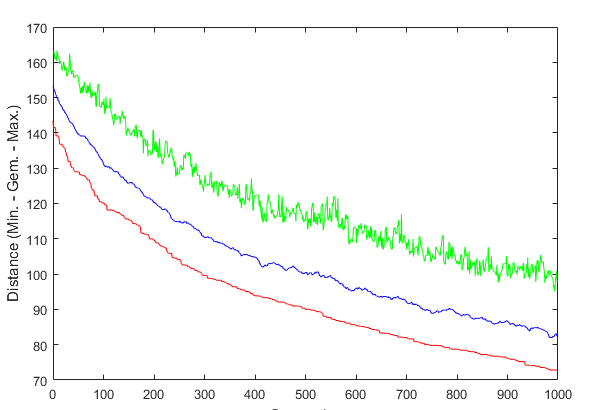
\includegraphics[width=1\textwidth]{../figures/question_5/FPS_off_gens.png}
      \caption{\textbf{Loop detection off}. \textbf{Best tour distance found: $\mathbf{72.79}$, computation time: 390 seconds}. } 
      \label{fig:fps_vraag5_off_gen}
\end{subfigure}
\hspace{0.05\textwidth}
\begin{subfigure}{0.45\textwidth}
  \centering
  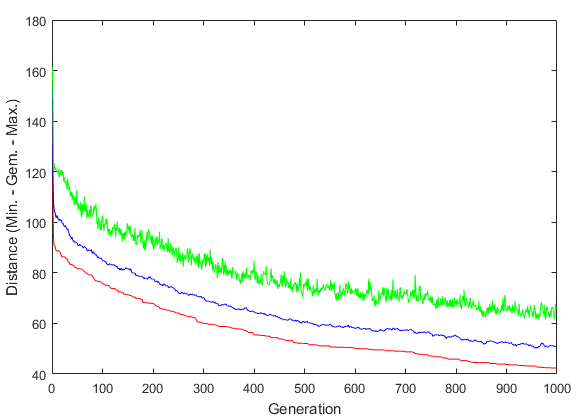
\includegraphics[width=1\textwidth]{../figures/question_5/FPS_on_gens.png}
      \caption{\textbf{Loop detection on}.  \textbf{Best tour distance found: $\mathbf{42.36}$, computation time: 431 seconds}.} 
      \label{fig:fps_vraag5_off_gen}
\end{subfigure}
\caption{The benchmark TSP problem \texttt{bcl380.tsp} with 380 cities is solved here using path representation with the following parameters: PR. MUT = $25\%$, PR. CROS = $60\%$ , ELITE = $5\%$. 200 individuals and 1000 generations.}
\label{fig:fps_gen}
\end{figure}

\begin{figure}[!]
\centering
 \scalebox{.5}{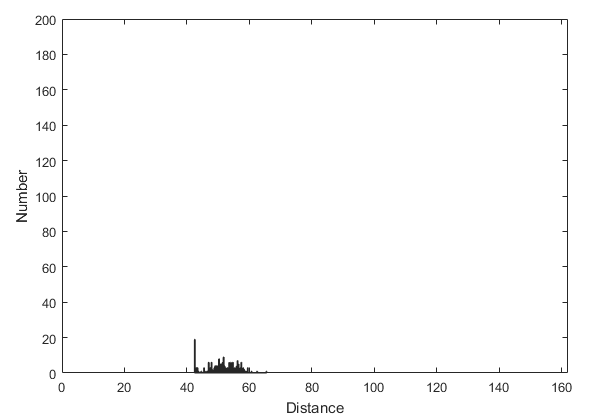
\includegraphics{../figures/question_5/FPS_hist.png}}
 
 \caption{Histogram at 1000 generations using path representations with fitness proportionate selection.}
 \label{fig:fps_hist}
\end{figure}


 \subsection{Tournament selection}
 Tournament selection selects parents by randomly choosing groups of n members of the population. From each group the individual with the best fitness value is selected as a parent. This continues until enough parents have been selected. For a full explanation we refer to \cite{handboek}.
 
 To test this selection mechanism the same method as in the previous section is used. From \ref{fig:tour_gen} it is clear that tournament selection does offer an improvement over the default rank selection. Worth noting is that tournament selection performs just as well with loop detection disabled as rank selection does with it enabled. A reason for this increased performance might be that tournament selection (with the right tournament size) strikes a good balance between selection pressure and sufficient probability for less fit members to survive, giving the algorithm greater chances of abandoning local optima that are not near the global optimum.
 
 A downside to the tournament selection is that after a large amount of generations, the variety in the population becomes extremely low. Figure \ref{fig:tourn_hist} shows over half of the population sitting at the same fitness (and thus likely representing the same tour). This reduces the effectiveness of the algorithm and might cause it to get stuck in a local optimum after all. The use of mechanisms to increase population diversity (e.g. supbpopulations) might give further improvements to the algorithm.
 
   \begin{figure}[!]
\centering
\begin{subfigure}{0.45\textwidth}
  \centering
  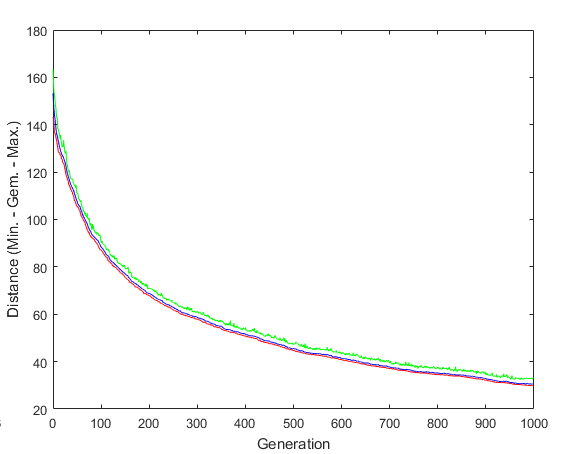
\includegraphics[width=1\textwidth]{../figures/question_5/tournament_off_gen.png}
      \caption{\textbf{Loop detection off}. \textbf{Best tour distance found: $\mathbf{26.79}$, computation time: 412 seconds}. } 
      \label{fig:tourn_vraag5_off_gen}
\end{subfigure}
\hspace{0.05\textwidth}
\begin{subfigure}{0.45\textwidth}
  \centering
  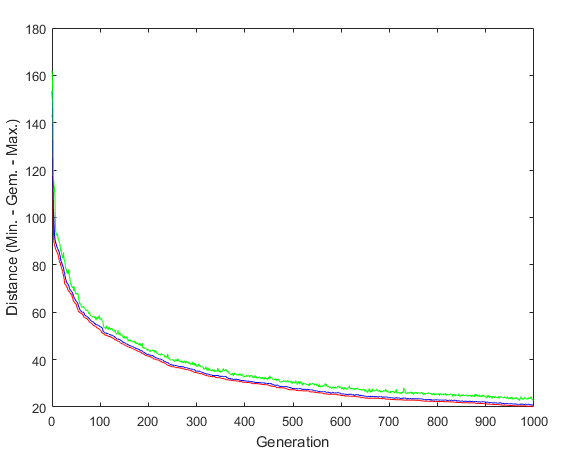
\includegraphics[width=1\textwidth]{../figures/question_5/tournament_on_on.png}
      \caption{\textbf{Loop detection on}.  \textbf{Best tour distance found: $\mathbf{20.21}$, computation time: 441 seconds}.} 
      \label{fig:tourn_vraag5_off_gen}
\end{subfigure}
\caption{The benchmark TSP problem \texttt{bcl380.tsp} with 380 cities is solved here using path representation and tournament selection with the following parameters: PR. MUT = $20\%$, PR. CROS = $60\%$ , ELITE = $5\%$, TOURN. SIZE = 5. 200 individuals and 1000 generations.}
\label{fig:tour_gen}
\end{figure}


\begin{figure}[!]
\centering
 \scalebox{.5}{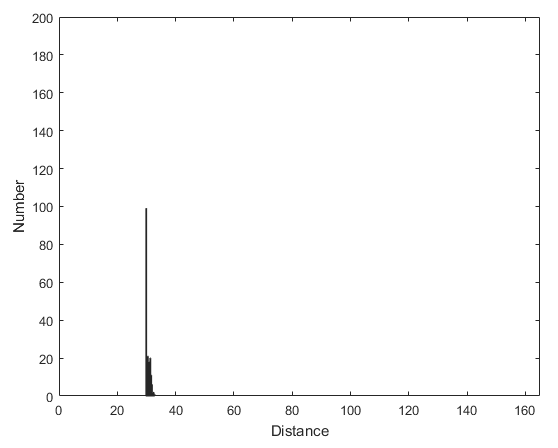
\includegraphics{../figures/question_5/tournament_off_hist.png}}
 
 \caption{Histogram at 1000 generations using path representations with tournament selection.}
 \label{fig:tourn_hist}
\end{figure}

\FloatBarrier
	\section{Conclusion}
	Unfortunately we have to conclude that we did not manage to make a large improvement to the genetic algorithm template. The use of path representation did only slightly improve fitness but not by much. Tournament selection does seem like a viable selection mechanism, resulting in a moderate improvement to the algorithm's performance. 
	That said, none of the methods we tested provided usefull solutions to TSP problems with a large amount of cities. Other representations and operators might perform better.
	
	\begin{thebibliography}{9}

\bibitem{handboek}
  A. E. Eiben, J.E. Smith,
  \emph{Introduction to Evolutionary Computing},
  Second Edition.

\end{thebibliography}
	\FloatBarrier
	


\begin{appendices}

%In de appendix bevind zich een deel van de code die gebruikt werd voor het bekomen van bovenstaande resultaten.
%De bijgevoegde code is tot een minimum gehouden, enkel de code die bijna volledig door onszelf 
%Het volledige project, inclusief de matlab bestanden om elk van bovenstaande resultaten te genereren kan gevonden worden op \href{https://github.com/double2double/wavelets}{https://github.com/double2double/wavelets}

In the appendices you can find a small part of the code that is used to obtain the results discussed in this report. To make sure that the appendix is not extremely long, only the code is shown that is completely written by ourselves. 

\section*{Matlab Code}


\subsection*{Implementation Order Crossover}
This function recombines two parents to create two children with the use of Order Crossover. 
\lstinputlisting{../code_appendix/order_crossover.m}


\subsection*{Implementation fitness function for path representation}
This function compute the fitness values corresponding to the candidate solutions in path representation.
\lstinputlisting{../code_appendix/tspfun_path.m}







%\lstinputlisting{../src/matlab/example_denoising.m}
%
%\subsection*{Code voor inpainting}
%\lstinputlisting{../src/matlab/inpainting_fun.m}
%\subsection*{Voorbeeld code voor gebruik van inpainting.}
%In onderstaand script word een afbeelding ingelezen en beschadigd met witte ruis. Nadien word het inpainting algoritme gebruikt om de ontbrekende pixelwaarden te schatten.
%\lstinputlisting{../src/matlab/example_inpainting.m}


\end{appendices}
	
	
\end{document}
